% !TEX spellckeck=en_GB

\section{Neural networks}\label{sec:ANN}

While the basis for the modern neural network was laid more than a hundred years ago, modern neural networks were proposed by \citet{McCulloch1943}. They described a computational structure analogous to a set of biological neurons. The premise is that a biological neuron accepts signals from many other adjacent neurons, and if it receives a large enough signal it fires, and emits a signal to those neurons it is connected to.  

Dubbed an artificial neural network (ANN) this computational analogue takes input from multiple sources, weights that input and produces an output if the signal from the weighted input is strong enough. A proper derivation will follow but for the moment we explore this simple intuition. These artificial neurons are ordered in layers, each successively passing information forward to a final output. Depending on the application, the output can be categorical or real-valued in nature. Each layer uses a matrix multiplication and a non-linear function to transform the input space in a way that condenses information, as most applications use transformations that reduce the dimensionality substantially before making a prediction.

A simple illustration of two neurons in one layer is provided in figure \ref{fig:ann_illustration}. In the figure the edges of the graph represent model parameters that are multiplied with the contents of the nodes they emerge from. At the recipient node the contributions from all the antecedent nodes are summed over, and "activated" with a non-linear function. In this way the artificial neuron is analogous to the activation of a biological neuron.

\begin{figure}[h]
\centering
\includegraphics{../figures/ann.pdf}
\caption[Fully connected neural network illustration]{An illustration of the graph constructed by two artificial neurons with three input nodes. The edges in the graph denote parameters that are multiplied with the node contents they emerge from. Colored edges show the flow of information from one input node to the predicted value. For details see the text.}\label{fig:ann_illustration}
\end{figure}


\noindent The ANN produces an output by what we call a forward pass. This defines all the mathematical operations from the input to the output of the network. More formally, let the input to an ANN be $\boldsymbol{x} \in \R^N$, and the matrix $\boldsymbol{W}^{[1]} \in \R^{N \times D}$ be a representation of the weight matrix forming the connections between the input and the artificial neurons, each layer has its own weights which we denote with bracketed superscripts. For a network with $n$ layers each layer then maintains a weight matrix 

\begin{align}
\boldsymbol{W}^{[l]} \; \forall \; l \in \{1,\, 2,\, \dots, n\},
\end{align}

\noindent which are used to transform the input to a space which enables regression or classification.  

Lastly we define the activation function $f(x)$ as a monotonic, once differentiable, function on $\R^1$. The function $f(x)$ determines the complexity of the neural network together with the number of neurons per layer and number of layers. The use of a non-linear activation is what allows for the ANN to represent more complex problems than we were able to with logistic and linear regression.

We are now ready to fully describe the forward pass, which transforms the input to an intermediate representation $\boldsymbol{a}$. The simplest such transformation is the fully connected, or \textit{dense}, layer. It bears close resemblance to the formulation of linear and logistic regression and is defined as 

\begin{equation}\label{eq:fwd}
	\boldsymbol{a}^{[1]} = f(\boldsymbol{x}\boldsymbol{W}^{[1]})_D,
\end{equation}

\noindent for the first layer in the network with inputs $\boldsymbol{x}$. In equation \ref{eq:fwd} the subscript, $D$, denotes that the function is applied element-wise on the output of dimension $\R^D$. 

Each node is additionally associated with a bias, ensuring that even zero valued weights in $\boldsymbol{W}^{[l]}$ can encode information. Let the bias for the layer be given as $\boldsymbol{b} \in \R^D$ in keeping with the notation above. Equation \ref{eq:fwd} then becomes

\begin{equation}\label{eq:fwd_b}
	\boldsymbol{a}^{[1]} = f(\boldsymbol{x}\boldsymbol{W}^{[1]} + \boldsymbol{b}^{[1]})_D.
\end{equation}

\noindent To tie the notation back to more traditional methods we note that if we only have one layer and a linear activation $f(x) = x$ the ANN becomes a formulation of a linear regression model. Keeping the linear regression formulation in mind we illustrate the difference by showing the full forward pass of a two-layer neural network, where we also introduce the output activation function $o(\cdot)$

\begin{align}
\boldsymbol{a}^{[1]} &= f(\boldsymbol{x}\boldsymbol{W}^{[1]}+ \boldsymbol{b}^{[1]})_D , \\
\boldsymbol{y} &= o(\boldsymbol{a}^{[1]}\boldsymbol{W}^{[2]} + \boldsymbol{b}^{[2]})_D .
\end{align}  

\noindent The difference between the intermediate representations $\boldsymbol{a}^{[l]}$ and the output $\boldsymbol{y}$ is largely semantic. However, we find it useful to separate the notations in an effort to provide clarity, and because the last layer of a network usually has an activation which differs from the rest of the network. This output activation $o(\cdot)$ is usually formulated depending on the analysis at hand. For regression tasks $o$ is commonly just a linear activation. Conversely for classification the logistic sigmoid is used for binary outcomes, or in the event of multiple classes we use the soft-max function. For a network with $n$ layers the soft-max function is defined as 

\begin{equation}\label{eq:softmax}
o(\boldsymbol{z})_i = \frac{e^{z_i^{[n]}}}{\sum_j e^{z_j^{[n]}}},
\end{equation}

\noindent where we introduce our notation for the input to the activation at each layer as $z_j^{[l]}$. We explicitly define this input as 

\begin{equation}\label{eq:fwd_multi}
	z_{j}^{[l]} = a^{[l-1]}_iW^{[l]}_{ij} + b^{[l]}_j,
\end{equation}

\noindent such that the intermediate representation as seen by the next layer is

\begin{equation}\label{eq:z}
a_j ^{[l]} = f(z_j^{[l]})_D.
\end{equation}

\noindent We seamlessly transition to a network of many layers $n$ which is a simple extension of the two-layer network presented above. A multi-layer network can then be described in terms of its forward pass as 

\begin{align}
\boldsymbol{a}^{[1]} &= f(\boldsymbol{x}\boldsymbol{W}^{[1]}+ \boldsymbol{b}^{[1]})_D , \\
\boldsymbol{a}^{[2]} &= f(\boldsymbol{a}^{[1]}\boldsymbol{W}^{[2]}+ \boldsymbol{b}^{[2]})_D , \\
&\vdots \\
\boldsymbol{y} &= o(\boldsymbol{a}^{[n-1]}\boldsymbol{W}^{[n]} + \boldsymbol{b}^{[n]})_D .
\end{align} 

\noindent Furthermore we note that the dimensions of the weight matrices are largely user specified, excepting the first dimension of $\boldsymbol{W}^{[1]}$ which maps to the input dimension, and the second dimension of the last layer which maps to the output. Otherwise the first dimension is chosen to fit with the previous output and the second is specified as a hyperparameter. Recall from section \ref{sec:hyperparams} that hyperparameters have to be specified and tuned outside the ordinary optimization procedure and are usually related to the complexity of the model and so cannot be arbitrarily chosen. 

We can now turn to the process of optimizing the model. In a neural network the variables that need to be fit are the elements of $\boldsymbol{W}^{[l]}$ that we denote $\wij^{[l]}$, and the biases which we denote with $b_j^{[l]}$. And while one can solve the linear regression optimization problem by matrix inversion, the multi-layer neural net does not have a closed form first derivative for $\wij^{[l]}$ or  $b_j^{[l]}$ because of the non-linearities between each layer. We are then forced to turn to iterative methods of the gradient, which we previously introduced in section \ref{sec:gd}

Based on whether the output is described by real values or a set of probabilities the cost takes on different forms, just as for linear and logistic regression. In the real case we use the now familiar mean squared error (MSE) cost, or in the event that we want to estimate a probability of an outcome; the binary cross-entropy. We discuss these cost-functions in general and especially the MSE and binary cross-entropy (BCE) earlier on in chapter \ref{chap:fundament}. Regardless of the cost the optimization problem is solved by a gradient descent procedure discussed in section \ref{sec:gd}. We we re-introduce the update form for the parameters as 

\begin{equation}\label{eq:nn_gd}
	\wij^{[l]} \leftarrow \wij^{[l]} -\eta \frac{\partial \mathcal{C}}{\partial \wij^{[l]}} .
\end{equation}

\subsection{Backpropagation}\label{sec:backpropagation}

In the vernacular of the machine learning literature the aim of the optimization procedure is to train the model to perform optimally on the regression, reconstruction or classification task at hand. Training the model requires the computation of the total derivative in equation \ref{eq:nn_gd}. This is also where the biological metaphor breaks down, as the brain is probably not employing gradient descent.

Backpropagation of errors by automatic differentiation, first described by \citet{Linnainmaa1976}, is a method of computing the partial derivatives required to go from the gradient of the loss to individual parameter derivatives. Conceptually we wish to describe the slope of the error in terms of our model parameters, but having multiple layers complicate this somewhat. 

The backpropagation algorithm begins with computing the total loss, here exemplified with the squared error function,
\begin{equation}\label{eq:tot_err}
	E = \mathcal{C}(\boldsymbol{\hat{y}}, \boldsymbol{y}) = \frac{1}{2n}\sum_n \sum_j (\hat{y}_{nj}-y_{nj} )^2.
\end{equation}

\noindent The factor one half is included for practical reasons to cancel the exponent under differentiation. As the gradient is multiplied by the learning rate $\eta$, this is ineffectual on the training itself. 

The sums over $n$ and $j$ enumerate the number of samples, and output dimensions respectively. Finding the update for the parameters then starts with taking the derivative of equation \ref{eq:tot_err} w.r.t the model output $y_j  = a^{[l]}_j$

\begin{equation}\label{eq:err_grad}
	\frac{\partial E}{\partial y_{j}} = \hat{y}_{j} - a^{[l]}_j.
\end{equation}

\noindent We have dropped the data index, as the differentiation is independent under the choice of data. In practice the derivative of each sample in the batch is averaged together for the gradient update of each parameter. 

The activation function, $f$, has classically been the logistic sigmoid function, but during the last decade the machine learning community has largely shifted to using the Rectified linear unit (ReLU). This shift was especially apparent after the success of \citet{Krizhevsky2012}. In this section we then exemplify the backpropagation algorithm with a network with ReLU activation. The ReLU function is defined in such a way that it is zero for all negative inputs and the identity otherwise, i.e. 

\begin{equation}\label{eq:relu}
	\text{ReLU} (x) = f(x) = \begin{cases}
	x, & \text{if } x > 0 \\
	0,  & \text{otherwise} .
	\end{cases}
\end{equation}

\noindent The ReLU is obviously monotonic and its derivative can be approximated with the Heaviside step-function which we denote with $H(x)$ and is mathematically expressed as 

\begin{equation}\label{eq:heaviside}
H(x) = f'(x) = 	\begin{cases}1, & \text{if } x > 0 \\
	0,  & \text{otherwise}.
\end{cases}
\end{equation}

\noindent Common to most neural network activations the computation of the derivative is very light-weight. In the case of the $ReLU$ function the computation of the derivative uses the mask needed to compute the activation itself, requiring no extra computing resources. 

It is important to note that the cost and activation as introduced in equations \ref{eq:tot_err}, \ref{eq:relu} and \ref{eq:heaviside} is not a be-all-end-all solution, but chosen for their ubiquitous nature in modern machine learning.

Returning to the optimization problem we start to unravel the backpropagation algorithm. We use equation \ref{eq:err_grad} to find the derivatives in terms of the last parameters, i.e. $\wij^{[n]}$ and $b_j^{[n]}$

\begin{align}
\frac{\partial E}{\partial \wij^{[n]}} &= 
\frac{\partial E}{\partial y_j} 
\frac{\partial y_j}{\partial z_j^{[n]}}
\frac{\partial z_j^{[n]}}{\partial \wij^{[n]}}, \\
&= \frac{\partial E}{\partial y_j} o'(z^{[n]}_j)
\frac{1}{\partial \wij^{[n]}} \left(a^{[n-1]}_iW^{[n]}_{ij} + b^{[n]}_j\right), \\
&= (\hat{y}_j - y_j)o'(z^{[n]}_j) a^{[n-1]}_i. \label{eq:backprop_w}
\end{align}

\noindent The differentiation of the error w.r.t to $b_j$ can be similarly derived to be 

\begin{equation}\label{eq:backprop_b}
\frac{\partial E}{\partial b_j^{[n]}}= (\hat{y}_j - y_j)o'(a^{[n]}_j).
\end{equation}

\noindent Repeating this procedure layer by layer is the process that defines the backpropagation algorithm. From equations \ref{eq:backprop_w} and \ref{eq:backprop_b} we discern a recursive pattern in the derivatives moving to the next layer. Before writing out the full backpropagation term we will introduce some more notation that makes bridging the gap to an implementation considerably simpler. From the repeating structure in the aforementioned equations we define the first operation needed for backpropagation,

\begin{equation}
\delta^n_j = (\hat{y}_j - y_j)o'(z_j^{[n]}).
\end{equation}

\noindent Note that this is an element-wise Hadamard product and not an implicit summation, expressed by the subscript index in $\hat{\delta}^n_j$.
The element-wise product of two matrices or vectors is denoted as  

\begin{equation}
\boldsymbol{a} \circ \boldsymbol{b}.
\end{equation}

\noindent This short-hand lets us define equations \ref{eq:backprop_w} and \ref{eq:backprop_b} in a more compact way

\begin{align}
\frac{\partial E}{\partial w_{ij}^{[n]}} &= \delta^n_j a^{[n-1]}_i,\\
\frac{\partial E}{\partial b_{j}^{[n]}} &= \delta^n_j.
\end{align} 

\noindent From the iterative nature of how we construct the forward pass we see that the last derivative in the chain for each layer, i.e. those in terms of the weights and biases, have the same form 

\begin{align}
\frac{\partial z_j^{[l]}}{\partial w_{ij}^{[l]}} &= a^{[l-1]}_i, \\
\frac{\partial z_j^{[l]}}{\partial b_{j}^{[l]}} &= 1.
\end{align}

\noindent These derivatives together with a general expression for the recurrent term $\delta^l_j$ are then the pieces we need to compute the parameter update rules. By summing up over the connecting nodes, $k$, to the layer, $l$, of interest $\delta_j^l$ can be expressed as

\begin{align}
\delta_j^l &= 
\sum_k \frac{\partial E}{\partial a_k^{[l+1]}} 
\frac{\partial a_k^{[l+1]}}{\partial z_k^{[l+1]}} 
\frac{\partial z_k^{[l+1]}}{\partial a_j^{[l]}} 
\frac{\partial a_j^{[l]}}{\partial z_j^{[l]}},\\
\delta_j^l &= 
\sum_k \delta^{l+1} \frac{\partial z_k^{[l+1]}}{\partial a_j^{[l]}} 
\frac{\partial a_j^{[l]}}{\partial z_j^{[l]}} \label{eq:penult_dl}.
\end{align}

\noindent From the definitions of the $z_j^{[l]}$ and $a_j^{[l]}$ terms we can then compute the last derivatives. These are then inserted back into \ref{eq:penult_dl}, giving a final expression for $\delta_j^l$,

\begin{equation}\label{eq:dl}
\delta_j^l = \sum_k \delta ^{l+1}_k w^{[l+1]}_{jk} f'(z_j^{[l]}).
\end{equation}

\noindent Finally the weight and bias update rules can then be written as 

\begin{align}
\frac{\partial E}{\partial w_{jm}^{[l]}} &= \delta_j^l a^{[l-1]}_m, \\
\frac{\partial E}{\partial b_{j}^{[l]}} &= \delta_j^l .
\end{align}

\noindent To finalize the discussion on the algorithm we illustrate how backpropagation might be implemented in algorithm \ref{algo:backprop}.

\begin{algorithm}
\caption{Backpropagation of errors in a fully connected neural network for a single sample $\boldsymbol{x}$.}\label{algo:backprop}
\KwData{Iterables 
 $\boldsymbol{a}^{[l]} $
 $\boldsymbol{z}^{[l]}$
 $\boldsymbol{W}^{[l]}$
 $\boldsymbol{b}^{[l]}$ 
$\forall \; l \in [1,\, 2,\, \dots ,\, n] $}
\KwIn{$\frac{\partial E}{\partial \boldsymbol{y}}$, $o'(\boldsymbol{z^{[n]}})$, $f'(\cdot)$}
\KwResult{Two iterables of the derivatives $\frac{\partial E}{\partial w_{ij}^{[l]}}$ and $\frac{\partial E}{\partial b_{j}^{[l]}}$ }
Initialization\;
$\delta_j^{n} \gets \frac{\partial E}{\partial \boldsymbol{y}} \circ o'(\boldsymbol{z^{[n]}})$\;
Compute derivatives\;  
\For{$l \in [n-1,\, \dots ,\, 1] $}{
	$\frac{\partial E}{\partial w_{jm}^{[l]}} \gets \hat{\delta}_j^{l+1} a^{[l]}_m$\;
	$\frac{\partial E}{\partial w_{jm}^{[l]}} \gets \hat{\delta}_j^{l+1}$\;
	$\delta_j^{l+1} \gets \sum_k \delta ^{l+1}_k w^{[l+1]}_{jk} f'(z_j^{[l]})$
}
\KwRet{$\frac{\partial E}{\partial w_{ij}^{[l]}}$ and $\frac{\partial E}{\partial b_{j}^{[l]}}$}
\end{algorithm}

The backward propagation framework is highly generalizable to variations of activation functions and network architectures. The two major advancements in the theory of ANNs are both predicated on being fully trainable by the backpropagation of errors. Before we consider these improvements made by the introduction of recurrent neural networks (RNN) and convolutional neural networks (CNN), we remark again on the strength of this algorithm. We are not only free to chose the activation function from a wide selection, the backpropagation algorithm also makes no assumptions on the transformation that constructs $z_j$. As long as it is once differentiable we are free to choose a different approach. This flexibility of the framework is part of the resurgent success of deep learning in the last decade. 

\subsection{Neural network architectures}

When creating a neural network on a computer with finite resources, a principled consideration must be made on the width and depth of the network. These terms are standard in machine learning literature and describe how many nodes per layer, and how many layers a network consists of respectively. A discussion of this consideration is neatly summarized in the work of \citet{Lin2017}. The authors provide strong reasoning for prioritizing deep networks over wide ones. They show that one can view many physical systems that generate the data a causal hierarchy (see figure 3 in \citet{Lin2017} for an illustration). This representation of stepwise transformations intuitively lends itself well to representation by a sequence of layers. This intuition builds on the fact that each layer contains a transformed, compressed, representation of the data. It is this bottleneck property of information compression that motivates the use of autoencoders, neural networks that compress and reconstruct the input when unlabelled data is plentiful and labelled data is scarce.

\subsection{Activation functions}\label{sec:activation}

Building neural networks depend in large part on the choice of the non-linearity that acts on the output from each layer. They are intrinsically tied to the attributes of the optimization scheme. Gradients have to pass backwards through all the layers to adjust the weights to make better predictions in the next iterations. In this section, we will discuss the attributes, strengths, and weaknesses of the four principal functions used as activations in neural networks. 

\subsubsection{Sigmoid activation functions}

Two sigmoid functions have been traditionally used in neural networks, and while they are now mostly of interest for educational purposes, they still see some use in niche models. Through logistic regression, we have already been introduced to the logistic sigmoid function. The logistic sigmoid was for the same reasons used in early classifying neural networks. Mathematically it has the form 

\begin{equation}
\sigma(x) = \frac{1}{1-e^{-x}}.
\end{equation}

\noindent As with the ReLU activation we introduced in the previous section the sigmoid activation has a derivative which is very cheap to compute, namely

\begin{equation}
\frac{d\sigma}{dx} = \sigma(x)(1 - \sigma(x))
\end{equation}

\noindent The second sigmoid activation is the hyperbolic tangent function. It saw widespread use at the start of the 2000s, especially in recurrent neural networks which we will discuss in greater detail later in this chapter. It is defined as 

\begin{equation}
\tanh x = \frac{e^x - e^{-x}}{e^x + e^{-x}}
\end{equation}

\noindent We observe that the hyperbolic tangent is simply a shifted and scaled version of the logistic sigmoid. Its derivative is slightly more expensive than for the logistic sigmoid, and it is given as 

\begin{equation}
\frac{d \tanh x}{d x}  = 1-\tanh^2 x
\end{equation}

\noindent The challenge with the sigmoid functions is that the gradient saturates. A saturated gradient occurs where there is little or no change in the values as a function of $x$. We illustrate the sigmoid activation functions in figure \ref{fig:sigmoid}. From this figure, we observe that for relatively small values, the gradient goes to zero, which makes optimization hard. Additionally, we note one of the convenient properties of the sigmoid functions; their values are capped. This property prohibits the gradient from exploding but also causes problems in the gradient. In the backwards propagation of errors, we multiply the contributions from the derivative of the cost at the preceding layers. As these are smaller than $1/4$ for the logistic sigmoid, the product can quickly vanish.  We also note that the logistic sigmoid is capped at zero, like the ReLU function, while the hyperbolic tangent is bounded at $-1$. The hyperbolic tangent then has the option to emit a bounded anti-signal.

\begin{figure}[ht]
\centering
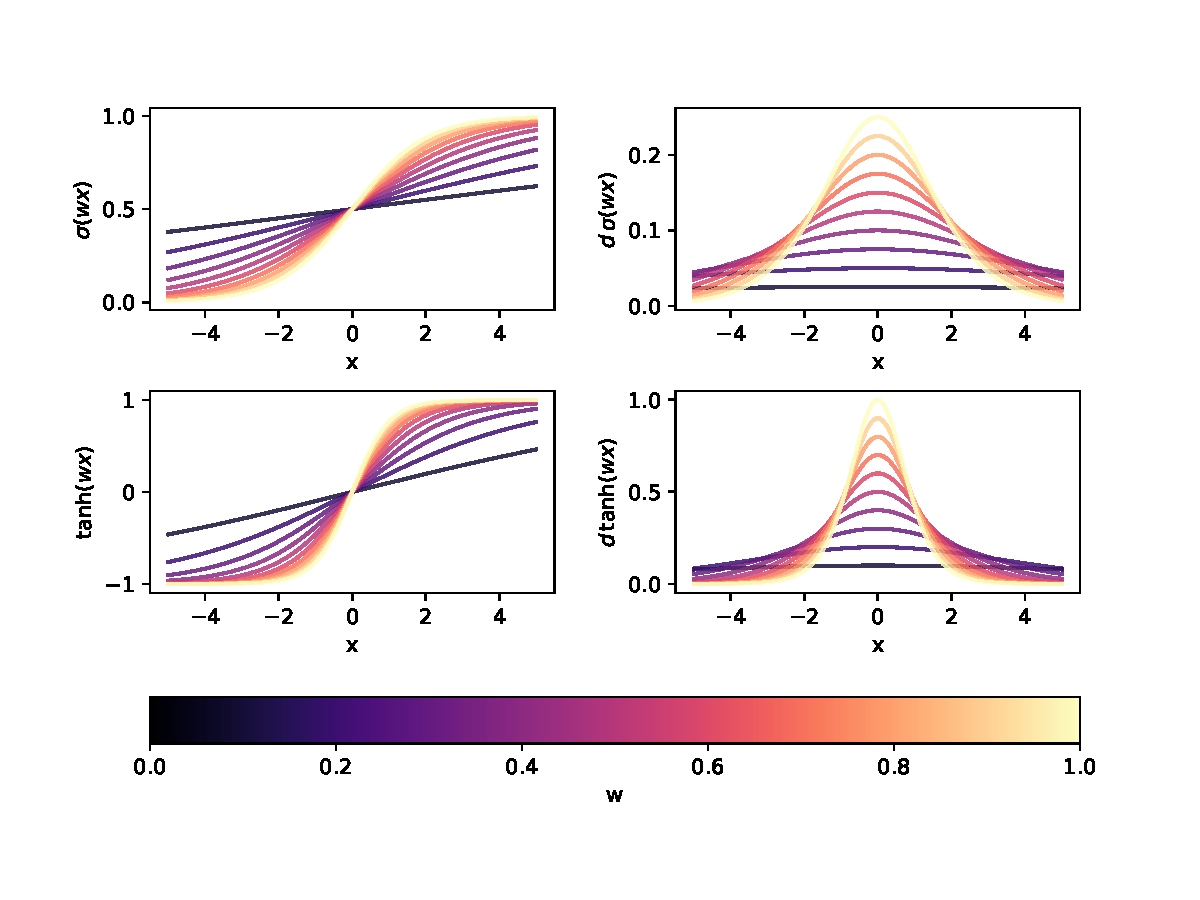
\includegraphics[width=0.8\textwidth, height=8cm]{../figures/activationssigmoids.pdf}
\caption[Sigmoid activation functions]{Sigmoid activation functions and their derivatives. The colorization indicates the value of the multiplicative weight $w$. The weight is multiplied with function argument $x$, which is what we differentiate with respect to.  We observe that the derivative deteriorates to zero as the function moves away from zero. The derivative going to zero means that a network using sigmoid activations generally struggle with saturated gradients which slows down training dramatically.}\label{fig:sigmoid}
\end{figure}

\subsubsection{Rectifiers}

On the other end of the scale rectified activations have gained traction in later years. We introduced the ReLU and its derivative in the previous section, but we will discuss a popular cousin here. The LReleaky rectified linear unit (LU) takes the ReLU and modifies it slightly by adding a small slope to the negative part of the activation. Mathematically we define the LReLU as 

\begin{equation}\label{eq:lrelu}
    \text{LReLU} (x)  = \begin{cases}
    x & \text{if } x > 0 \\
    \alpha\cdot x  & \text{otherwise},
    \end{cases}
\end{equation}

\noindent where $\alpha$ is a small positive real number. The differentiation of the LReLU is then 

\begin{equation}\label{eq:lrelu}
    \frac{d}{dx}\text{LReLU} (x) = \begin{cases}
    1 & \text{if } x > 0 \\
    \alpha & \text{otherwise}.
    \end{cases}
\end{equation}

\noindent Immediately it becomes clear that for the rectifier functions we have the opposite problem from what we encountered for the sigmoid activations. As the derivative is non-zero for a large range of values, we no longer have a concern for saturated gradients. We are also safe from the activation contributing to exploding or vanishing gradients as the derivative is equal to one. We illustrate the defining features of the rectifiers in figure \ref{fig:elu}

\begin{figure}[ht]
\centering
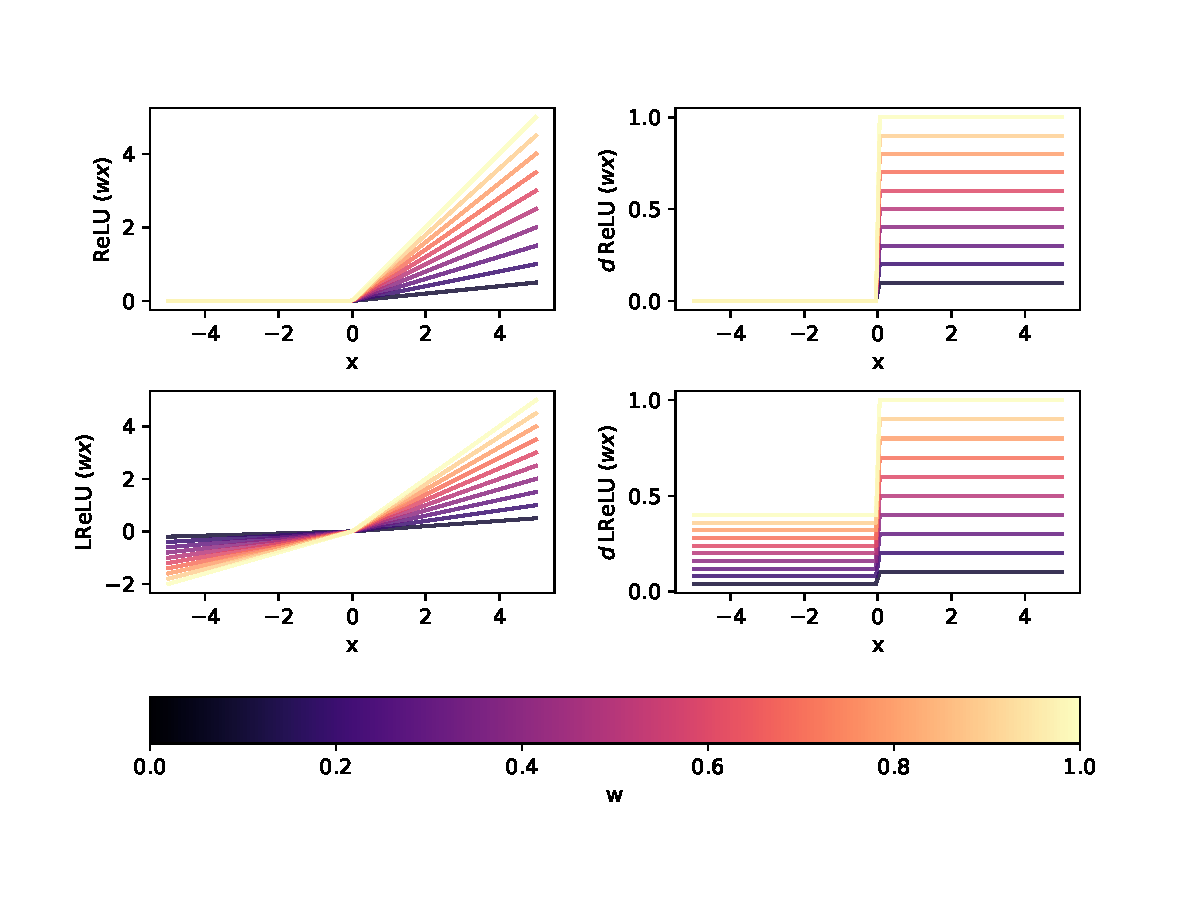
\includegraphics[width=0.8\textwidth, height=8cm]{../figures/activationselus.pdf}
\caption[Rectifier activation functions]{Rectifier activation functions and their derivatives, the colorization indicates that the function is multiplied with a second variable. In contrast with the sigmoid activations the derivative is non-zereo in $\R^+$ for the ReLU and non-zero on the entirety of $\R$ for the LReLU.}\label{fig:elu}
\end{figure}

One heuristic method of handling exploding gradients that has seen wide applications is gradient capping. When computing the gradients, one chooses a maximum value for e.g., the norm of the gradient of a layer and shrink any update that crosses that threshold. The downside of this is that it can slow down training substantially. More elegant solutions are usually employed in conjunction with a capped gradient which we will discuss in the next section on the regularization of neural networks. 


\section{Deep learning regularization}

As neural networks can be made arbitrarily complex, reducing the degree of over-fitting is an important concern. Regularization of deep learning uses both tried and true algorithms, as we discussed in chapter \ref{chap:fundament}, and some specialized tools developed for use with neural networks specifically. 

Traditional measures of regularization like using cross-validation and weight constraints are both important features of reducing overfitting in deep learning algorithms. We introduced cross-validation in section \ref{sec:cv} as a way to estimate appropriate model complexities. Cross-validation is model agnostic and can be applied to estimate an appropriate complexity for an arbitrary model or the optimal values for the gradient descent hyperparameters. 

Weight constraints are similarly convenient additions to the cost function. The only modification required from equation \ref{eq:mse_ridge} is adding a summation term over the layers. For a $L_2$ regularized neural net the cost function can then be written as 

\begin{equation}
C(\hat{y}_i, f(\boldsymbol{x}_i; \theta)) = (\hat{y}_i - f(\boldsymbol{x}_i; \theta))^2 + \lambda\sum_{lij}||w_{ij}^{[l]}||^2_2.
\end{equation}

\noindent More specific tools for neural networks have been developed in later years, and we will discuss two of these that has seen extensive application in recent works. 

\subsubsection{Dropout}\label{sec:dropout}

Armed with the knowledge that neural networks are usually more complex than the problem at hand warrants, \citet{Srivastava2014} proposes a wonderfully simple remedy: dropout. The premise is simple: after the activation of a layer, randomly set $d$ of these activations to zero. The fraction of the activations that $d$ represents is called the dropout-rate and is typically chosen to be a few tenths. Dropout adds a regularizing effect by having the network increase the redundancy of its prediction and thus forcibly reducing the complexity of the network. 

\subsubsection{Batch Normalization}\label{sec:batchnorm}

The second addition we discuss more directly addresses a problem in the optimization, and adds a regularizing effect only as a bi-product of the intended purpose. Batch normalization was introduced by \citet{Ioffe2015} as a means to address the internal covariance shift in neural networks. 

Conceptually one can think of the challenge presented by an internal covariance shift as an unintended consequence of the gradient descent procedure. When adjusting weights in a layer its gradients, we do not adjust them with respect to the change in the weights of the preceding layers. This slows down training substantially and is what \citet{Ioffe2015} describes as the internal covariance shift. To reduce the effects of this problem the authors propose to scale and center the outputs of each layer, before feeding it to the next in line. The normalization happens over each batch of training data and consists of two steps. Let the output from a layer be given as $a_k^{[l]}$ in keeping with previous notation. Furthermore, let the samples in a batch be indicated by the index $i$. Thus the activations can be denoted as a matrix $a_{ik}^{[l]}$. The batch normalization procedure then begins by computing the batch-wise mean, $\mu_k$, per feature $k$ for a batch of size $n$ 

\begin{equation}
\mu_k = \frac{1}{n} \sum_i^n a_{ik}^{[l]}.
\end{equation}

\noindent Secondly we compute the variance of the feature as 

\begin{equation}
\sigma_k^2= \sum_i (a^{[l]}_{ik} - \mu_k)^2.
\end{equation}

\noindent We can then compute the normalized activations using the mean and variance of the features, mathematically these are given as

\begin{equation}
\hat{a}_{ik}^{[l]} = \frac{\hat{a}_{ik}^{[l]} - \mu_k}{\sqrt{\sigma_k^2 + \epsilon}},
\end{equation}

\noindent where $\epsilon$ is a small number large enough to make the denominator non-zero, usually $\epsilon = \num{1e-8}$. The final part of the batch normalization procedure is to let the network determine a scale and shift of the new features, adding new features to the gradient descent procedure. The final expression for the features being fed forward is then 

\begin{equation}\label{eq:bn}
\text{BN}_{\gamma, \beta}(a_{ik}^{[l]}) = \gamma  \hat{a}_{ik}^{[l]} + \beta.
\end{equation} 

\noindent The primary effect of batch normalization is then to speed up training. \citet{Ioffe2015} shows that orders of magnitude larger learning rates may be used in experiments. Additionally, there is a contribution to the regularization by providing non-deterministic outputs as the normalization parameters are dependent on the other samples in a batch. 

As a bonus effect, the procedure lessens the potential problems with exploding and vanishing gradients: By placing the normalization layer before a sigmoid layer the probability of the activations being in the active region of the functions increases. Conversely, for the rectifier units placing the normalization after the activation lessens the chance for an exploding value in the gradient.

For all the merits of batch normalization, a fundamental challenge still remains. Since the normalization is over the feature axis, it adds a substantial number of parameters. For models who heavily use normalization, the scale and shift parameters can add up to $20\%-30\%$ of the weights in a model. Additionally, we observe that the computation involves a square root and a squaring operation which principally necessitates a full $64$ bit precision in the floating-point computation. 